\documentclass[border=5mm]{standalone}
\usepackage[T1]{fontenc}
\usepackage{helvet}
\renewcommand{\familydefault}{\sfdefault}
\usepackage{tikz}
\usepackage{amsmath,amssymb}
\usetikzlibrary{calc,positioning,arrows.meta,shadows.blur,fit,shapes.geometric,
                 decorations.pathmorphing,backgrounds}

% ══════════════════════════════════════════════════════════════
% PALETTE — refined for high-impact scientific figure
% ══════════════════════════════════════════════════════════════
\definecolor{L1}{HTML}{0D47A1}
\definecolor{L1bg}{HTML}{E3F2FD}
\definecolor{L2}{HTML}{00695C}
\definecolor{L2bg}{HTML}{E0F2F1}
\definecolor{L3}{HTML}{E65100}
\definecolor{L3bg}{HTML}{FFF3E0}
\definecolor{L4}{HTML}{6A1B9A}
\definecolor{L4bg}{HTML}{F3E5F5}
\definecolor{gold}{HTML}{F9A825}
\definecolor{dk}{HTML}{212121}
\definecolor{mg}{HTML}{616161}
\definecolor{ac}{HTML}{37474F}
\definecolor{sg}{HTML}{2E7D32}
\definecolor{wr}{HTML}{C62828}
\definecolor{cy}{HTML}{00838F}
\definecolor{pk}{HTML}{AD1457}

\tikzset{
  layer/.style={rounded corners=10pt, draw=#1, line width=2pt, fill=#1!6, inner sep=0pt},
  badge/.style={circle, minimum size=32pt, font=\bfseries\Large\sffamily, fill=#1, text=white, inner sep=0pt,
    blur shadow={shadow blur steps=5, shadow xshift=1pt, shadow yshift=-1.5pt, shadow opacity=25}},
  ltitle/.style={font=\bfseries\LARGE\sffamily, text=#1},
  lsub/.style={font=\large\sffamily, text=#1!70!black},
  keyeq/.style={rounded corners=6pt, draw=#1, line width=1.2pt, fill=white, inner sep=10pt,
    blur shadow={shadow blur steps=3, shadow xshift=0.5pt, shadow yshift=-0.5pt, shadow opacity=18}},
  pill/.style={rounded corners=12pt, draw=#1!60!black, line width=0.8pt, fill=#1!12, inner sep=8pt,
    font=\normalsize\sffamily, text=dk, minimum height=28pt},
  bigarrow/.style={-{Triangle[length=10pt,width=8pt]}, line width=3.5pt, ac},
  gtside/.style={-{Triangle[length=8pt,width=6pt]}, line width=2.5pt, gold, dashed, dash pattern=on 6pt off 4pt},
  cnode/.style={circle, minimum size=26pt, font=\bfseries\small\sffamily, fill=#1!20, draw=#1, line width=1.2pt, inner sep=0pt},
  starbox/.style={rounded corners=8pt, draw=L4, line width=2.5pt, fill=white,
    blur shadow={shadow blur steps=6, shadow xshift=1pt, shadow yshift=-2pt, shadow opacity=30}},
  imgbox/.style={rounded corners=4pt, draw=#1!50, line width=0.8pt, fill=#1!5, inner sep=3pt},
}

\begin{document}
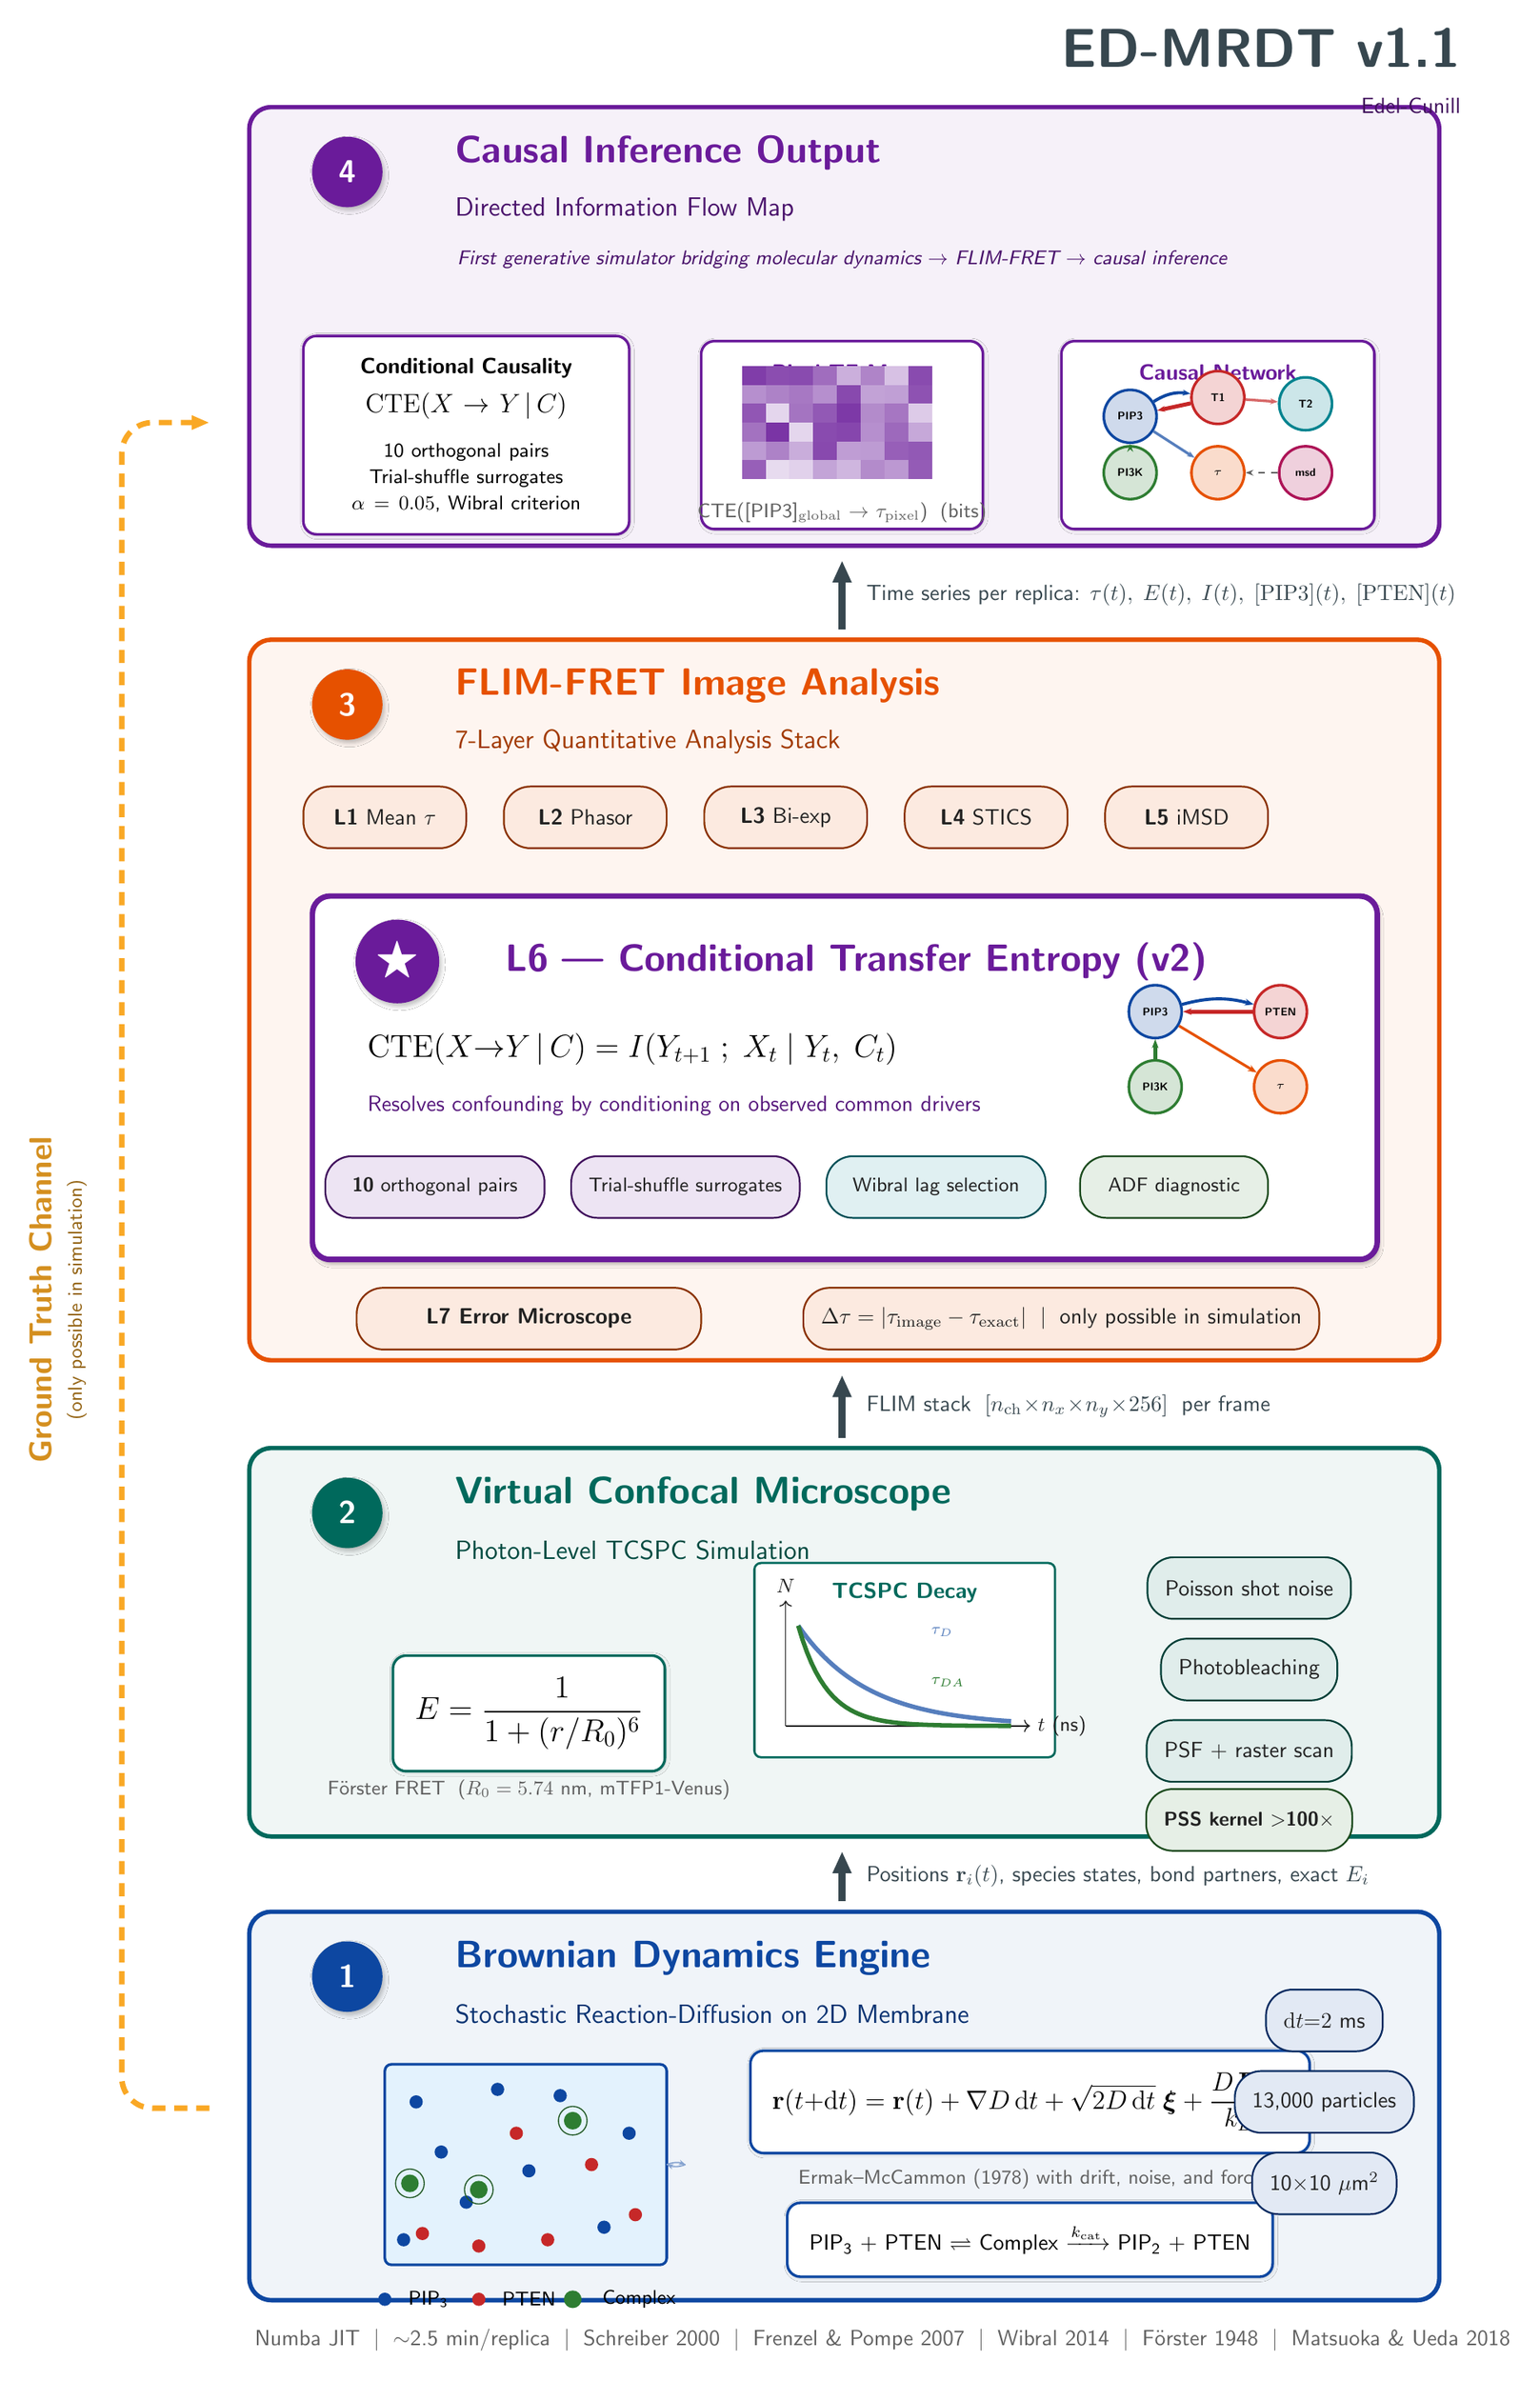
\begin{tikzpicture}[x=1cm, y=1cm]

\def\W{19}
\def\C{9.5}

% Layer positions and heights
\def\Ya{0}     \def\Ha{6.2}
\def\Yb{7.4}   \def\Hb{6.2}
\def\Yc{15.0}  \def\Hc{11.5}
\def\Yd{28.0}  \def\Hd{7.0}

% ================================================================
% LAYER 1 — BROWNIAN DYNAMICS
% ================================================================
\node[layer=L1, minimum width=\W cm, minimum height=\Ha cm, anchor=south west] (C1) at (0,\Ya) {};

\node[badge=L1] at (1.6, \Ya+\Ha-1.0) {\textsf{1}};
\node[ltitle=L1, anchor=west] at (3.2, \Ya+\Ha-0.7) {Brownian Dynamics Engine};
\node[lsub=L1, anchor=west] at (3.2, \Ya+\Ha-1.6) {Stochastic Reaction-Diffusion on 2D Membrane};

% Membrane schematic — improved with periodic boundary markers
\begin{scope}[shift={(2.2, \Ya+0.6)}]
  \draw[L1, line width=1.2pt, rounded corners=3pt, fill=L1bg] (0,0) rectangle (4.5,3.2);
  % PIP3 (blue)
  \foreach \x/\y in {0.5/2.6, 1.3/1.0, 2.8/2.7, 3.5/0.6, 3.9/2.1, 0.9/1.8, 2.3/1.5, 1.8/2.8, 0.3/0.4} {
    \fill[L1] (\x,\y) circle (3pt); }
  % PTEN (red)
  \foreach \x/\y in {0.6/0.5, 2.1/2.1, 3.3/1.6, 2.6/0.4, 1.5/0.3, 4.0/0.8} {
    \fill[wr] (\x,\y) circle (3pt); }
  % Complexes (green with ring)
  \foreach \x/\y in {1.5/1.2, 3.0/2.3, 0.4/1.3} {
    \fill[sg] (\x,\y) circle (4pt);
    \draw[sg!70!black, line width=0.5pt] (\x,\y) circle (6.5pt); }
  % Periodic boundary arrows
  \draw[L1!50, line width=0.6pt, -{Stealth[length=3pt]}] (4.5,1.6) to[bend left=20] (4.8,1.6);
  \draw[L1!50, line width=0.6pt, -{Stealth[length=3pt]}] (4.8,1.6) to[bend left=20] (4.5,1.6);
  % Legend
  \fill[L1] (0.0,-0.55) circle (3pt);
  \node[font=\small\sffamily, anchor=west] at (0.25,-0.55) {PIP\textsubscript{3}};
  \fill[wr] (1.5,-0.55) circle (3pt);
  \node[font=\small\sffamily, anchor=west] at (1.75,-0.55) {PTEN};
  \fill[sg] (3.0,-0.55) circle (4pt);
  \node[font=\small\sffamily, anchor=west] at (3.35,-0.55) {Complex};
\end{scope}

% Langevin equation — centered better
\node[keyeq=L1, font=\large] (eq1) at (12.5, \Ya+3.2)
  {$\mathbf{r}(t{+}\mathrm{d}t) = \mathbf{r}(t) + \nabla D\,\mathrm{d}t + \sqrt{2D\,\mathrm{d}t}\;\boldsymbol{\xi} + \dfrac{D\,\mathbf{F}\,\mathrm{d}t}{k_BT}$};
\node[font=\small\sffamily, text=mg, anchor=north] at (12.5, \Ya+2.25)
  {Ermak--McCammon (1978) with drift, noise, and force};

% Reaction network
\node[keyeq=L1, font=\normalsize] at (12.5, \Ya+1.0)
  {PIP\textsubscript{3} + PTEN $\rightleftharpoons$ Complex $\xrightarrow{k_\mathrm{cat}}$ PIP\textsubscript{2} + PTEN};

\node[pill=L1] at (17.2, \Ya+4.5) {$\mathrm{d}t{=}2$ ms};
\node[pill=L1] at (17.2, \Ya+3.2) {13{,}000 particles};
\node[pill=L1] at (17.2, \Ya+1.9) {10$\times$10 $\mu$m$^2$};

% ================================================================
% ARROW 1 → 2
% ================================================================
\draw[bigarrow] (\C, \Ya+\Ha+0.2) -- (\C, \Yb-0.2)
  node[midway, right=6pt, font=\normalsize\sffamily, text=ac]
  {Positions $\mathbf{r}_i(t)$, species states, bond partners, exact $E_i$};

% ================================================================
% LAYER 2 — VIRTUAL MICROSCOPE
% ================================================================
\node[layer=L2, minimum width=\W cm, minimum height=\Hb cm, anchor=south west] (C2) at (0,\Yb) {};

\node[badge=L2] at (1.6, \Yb+\Hb-1.0) {\textsf{2}};
\node[ltitle=L2, anchor=west] at (3.2, \Yb+\Hb-0.7) {Virtual Confocal Microscope};
\node[lsub=L2, anchor=west] at (3.2, \Yb+\Hb-1.6) {Photon-Level TCSPC Simulation};

% FRET equation
\node[keyeq=L2, font=\Large] (eqf) at (4.5, \Yb+2.0)
  {$E = \dfrac{1}{1 + (r/R_0)^6}$};
\node[font=\small\sffamily, text=mg, anchor=north] at (eqf.south)
  {F\"orster FRET\; ($R_0 = 5.74$ nm, mTFP1-Venus)};

% TCSPC decay curve
\begin{scope}[shift={(10.5, \Yb+1.8)}]
  \draw[L2, line width=1pt, rounded corners=3pt, fill=white] (-2.4,-0.5) rectangle (2.4,2.6);
  \node[font=\normalsize\sffamily\bfseries, text=L2, anchor=north] at (0,2.4) {TCSPC Decay};
  \draw[dk, line width=0.5pt, ->] (-1.9,0) -- (2.0,0) node[right, font=\small] {$t$ (ns)};
  \draw[dk, line width=0.5pt, ->] (-1.9,0) -- (-1.9,2.0) node[above, font=\small] {$N$};
  % Donor-only (blue, slow decay)
  \draw[L1!70, line width=2pt, domain=-1.7:1.7, samples=50]
    plot (\x, {1.6*exp(-0.9*(\x+1.7))});
  % Donor+FRET (green, fast decay)
  \draw[sg, line width=2pt, domain=-1.7:1.7, samples=50]
    plot (\x, {1.6*exp(-2.2*(\x+1.7))});
  % Legend
  \node[font=\scriptsize\sffamily, text=L1!70, anchor=west] at (0.3, 1.5) {$\tau_D$};
  \node[font=\scriptsize\sffamily, text=sg, anchor=west] at (0.3, 0.7) {$\tau_{DA}$};
\end{scope}

% Noise/process pills
\node[pill=L2] at (16.0, \Yb+4.0) {Poisson shot noise};
\node[pill=L2] at (16.0, \Yb+2.7) {Photobleaching};
\node[pill=L2] at (16.0, \Yb+1.4) {PSF + raster scan};

% PSS speedup
\node[pill=sg, font=\small\sffamily\bfseries] at (16.0, \Yb+0.3) {PSS kernel $>$100$\times$};

% ================================================================
% ARROW 2 → 3
% ================================================================
\draw[bigarrow] (\C, \Yb+\Hb+0.2) -- (\C, \Yc-0.2)
  node[midway, right=6pt, font=\normalsize\sffamily, text=ac]
  {FLIM stack\; $[n_\mathrm{ch} \!\times\! n_x \!\times\! n_y \!\times\! 256]$\; per frame};

% ================================================================
% LAYER 3 — FLIM-FRET ANALYSIS
% ================================================================
\node[layer=L3, minimum width=\W cm, minimum height=\Hc cm, anchor=south west] (C3) at (0,\Yc) {};

\node[badge=L3] at (1.6, \Yc+\Hc-1.0) {\textsf{3}};
\node[ltitle=L3, anchor=west] at (3.2, \Yc+\Hc-0.7) {FLIM-FRET Image Analysis};
\node[lsub=L3, anchor=west] at (3.2, \Yc+\Hc-1.6) {7-Layer Quantitative Analysis Stack};

% L1-L5 analysis pills
\pgfmathsetmacro{\pillY}{\Yc+\Hc-2.8}
\node[pill=L3, minimum width=2.6cm] at (2.2, \pillY) {\textbf{L1} Mean $\tau$};
\node[pill=L3, minimum width=2.6cm] at (5.4, \pillY) {\textbf{L2} Phasor};
\node[pill=L3, minimum width=2.6cm] at (8.6, \pillY) {\textbf{L3} Bi-exp};
\node[pill=L3, minimum width=2.6cm] at (11.8, \pillY) {\textbf{L4} STICS};
\node[pill=L3, minimum width=2.6cm] at (15.0, \pillY) {\textbf{L5} iMSD};

% ════════════════════════════════════════════════════════
% L6 CONDITIONAL TRANSFER ENTROPY — THE STAR (updated v2)
% ════════════════════════════════════════════════════════
\node[starbox, minimum width=17cm, minimum height=5.8cm,
      anchor=south west] (TEbox) at (1.0, \Yc+1.6) {};

% Star badge
\node[badge=L4, minimum size=38pt, font=\bfseries\huge] at (2.4, \Yc+6.4) {$\bigstar$};

% Title — updated to CTE v2
\node[font=\bfseries\LARGE\sffamily, text=L4, anchor=west] at (4.0, \Yc+6.4)
  {L6 --- Conditional Transfer Entropy (v2)};

% THE CTE equation — the core upgrade
\node[font=\Large, anchor=west] at (1.8, \Yc+5.0)
  {$\mathrm{CTE}(X{\to}Y\,|\,C) = I\!\left(Y_{t+1}\;;\;X_t\;\middle|\;Y_t,\;C_t\right)$};

% Explanation
\node[font=\normalsize\sffamily, text=L4!80!black, anchor=west] at (1.8, \Yc+4.1)
  {Resolves confounding by conditioning on observed common drivers};

% Feature pills inside TE box
\node[pill=L4, minimum width=3.5cm, font=\small\sffamily] at (3.0, \Yc+2.8)
  {\textbf{10} orthogonal pairs};
\node[pill=L4, minimum width=3.5cm, font=\small\sffamily] at (7.0, \Yc+2.8)
  {Trial-shuffle surrogates};
\node[pill=cy, minimum width=3.5cm, font=\small\sffamily] at (11.0, \Yc+2.8)
  {Wibral lag selection};
\node[pill=sg, minimum width=3.0cm, font=\small\sffamily] at (14.8, \Yc+2.8)
  {ADF diagnostic};

% Causal network — updated with PIP3-PTEN species
\begin{scope}[shift={(15.5, \Yc+5.0)}]
  \node[cnode=L1, minimum size=24pt] (nPIP3) at (-1.0, 0.6) {\tiny PIP3};
  \node[cnode=wr, minimum size=24pt] (nPTEN) at (1.0, 0.6) {\tiny PTEN};
  \node[cnode=sg, minimum size=24pt] (nPI3K) at (-1.0, -0.6) {\tiny PI3K};
  \node[cnode=L3, minimum size=24pt] (ntau) at (1.0, -0.6) {\tiny $\tau$};
  % Arrows — key causal directions
  \draw[-{Stealth[length=4pt]}, wr, line width=1.8pt] (nPTEN) -- (nPIP3);
  \draw[-{Stealth[length=4pt]}, L1, line width=1.4pt] (nPIP3) to[bend left=15] (nPTEN);
  \draw[-{Stealth[length=4pt]}, sg, line width=1.6pt] (nPI3K) -- (nPIP3);
  \draw[-{Stealth[length=4pt]}, L3, line width=1.2pt] (nPIP3) -- (ntau);
\end{scope}

% L7 Error Microscope
\node[pill=L3, minimum width=5.5cm, font=\normalsize\sffamily\bfseries] at (4.5, \Yc+0.7)
  {\textbf{L7} Error Microscope};
\node[pill=L3, minimum width=7cm] at (13.0, \Yc+0.7)
  {$\Delta\tau = |\tau_\mathrm{image} - \tau_\mathrm{exact}|$ \;\textbar\; only possible in simulation};

% ================================================================
% ARROW 3 → 4
% ================================================================
\draw[bigarrow] (\C, \Yc+\Hc+0.2) -- (\C, \Yd-0.2)
  node[midway, right=6pt, font=\normalsize\sffamily, text=ac]
  {Time series per replica: $\tau(t),\; E(t),\; I(t),\; [\mathrm{PIP3}](t),\; [\mathrm{PTEN}](t)$};

% ================================================================
% LAYER 4 — CAUSAL INFERENCE OUTPUT
% ================================================================
\node[layer=L4, minimum width=\W cm, minimum height=\Hd cm, anchor=south west] (C4) at (0,\Yd) {};

\node[badge=L4] at (1.6, \Yd+\Hd-1.0) {\textsf{4}};
\node[ltitle=L4, anchor=west] at (3.2, \Yd+\Hd-0.7) {Causal Inference Output};
\node[lsub=L4, anchor=west] at (3.2, \Yd+\Hd-1.6) {Directed Information Flow Map};

% Tagline
\node[font=\small\sffamily\itshape, text=L4!70!black]
  at (\C, \Yd+4.6)
  {First generative simulator bridging molecular dynamics $\to$ FLIM-FRET $\to$ causal inference};

% TE results panel
\begin{scope}[shift={(3.5, \Yd+1.8)}]
  \node[keyeq=L4, text width=4.5cm, align=center, minimum height=3.0cm] at (0,0) {%
    {\bfseries\normalsize Conditional Causality}\\[6pt]
    {\large $\mathrm{CTE}(X \!\to\! Y \,|\, C)$}\\[8pt]
    {\small 10 orthogonal pairs}\\
    {\small Trial-shuffle surrogates}\\
    {\small $\alpha = 0.05$, Wibral criterion}
  };
\end{scope}

% TE pixel heatmap placeholder
\begin{scope}[shift={(9.5, \Yd+1.8)}]
  \node[keyeq=L4, minimum width=4.5cm, minimum height=3.0cm] at (0,0) {};
  \node[font=\normalsize\sffamily\bfseries, text=L4, anchor=north] at (0,1.25) {Pixel TE Map};
  % Heatmap grid with varying intensities
  \foreach \i in {0,...,7} {
    \foreach \j in {0,...,5} {
      \pgfmathsetmacro{\v}{int(15+rnd*75)}
      \fill[L4!\v] (-1.6+\i*0.38, -0.7+\j*0.3) rectangle (-1.6+\i*0.38+0.38, -0.7+\j*0.3+0.3);
    }
  }
  \node[font=\small\sffamily, text=mg, anchor=north] at (0,-0.95)
    {CTE([PIP3]$_\mathrm{global}$ $\to$ $\tau_\mathrm{pixel}$) \;(bits)};
\end{scope}

% Causal Network — large, with all 10 pairs
\begin{scope}[shift={(15.5, \Yd+1.8)}]
  \node[keyeq=L4, minimum width=5.0cm, minimum height=3.0cm] at (0,0) {};
  \node[font=\normalsize\sffamily\bfseries, text=L4, anchor=north] at (0,1.25) {Causal Network};
  % Nodes
  \node[cnode=L1, minimum size=24pt] (cPIP3) at (-1.4, 0.3) {\tiny PIP3};
  \node[cnode=wr, minimum size=24pt] (cPTEN) at (0.0, 0.6) {\tiny T1};
  \node[cnode=cy, minimum size=24pt] (cT2)   at (1.4, 0.5) {\tiny T2};
  \node[cnode=sg, minimum size=24pt] (cPI3K) at (-1.4, -0.6) {\tiny PI3K};
  \node[cnode=L3, minimum size=24pt] (ctau)  at (0.0, -0.6) {\tiny $\tau$};
  \node[cnode=pk, minimum size=24pt] (cMSD)  at (1.4, -0.6) {\tiny msd};
  % Edges — significant pairs get green, expected-null get gray dashed
  \draw[-{Stealth[length=3.5pt]}, wr, line width=1.8pt] (cPTEN) -- (cPIP3);
  \draw[-{Stealth[length=3.5pt]}, L1, line width=1.4pt] (cPIP3) to[bend left=20] (cPTEN);
  \draw[-{Stealth[length=3.5pt]}, sg, line width=1.6pt] (cPI3K) -- (cPIP3);
  \draw[-{Stealth[length=3.5pt]}, wr!70, line width=1.2pt] (cPTEN) -- (cT2);
  \draw[-{Stealth[length=3.5pt]}, L1!70, line width=1.2pt] (cPIP3) -- (ctau);
  \draw[-{Stealth[length=3.5pt]}, mg, line width=0.6pt, dashed] (cMSD) -- (ctau);
\end{scope}

% ================================================================
% GROUND TRUTH BYPASS — the unique capability
% ================================================================
\draw[gtside, rounded corners=14pt]
  (-0.6, \Ya+\Ha*0.5) -- (-2.0, \Ya+\Ha*0.5)
  -- (-2.0, \Yd+2.0) -- (-0.6, \Yd+2.0);
\node[rotate=90, font=\Large\sffamily\bfseries, text=gold!85!black, anchor=south]
  at (-3.0, 16) {Ground Truth Channel};
\node[rotate=90, font=\small\sffamily, text=gold!60!black, anchor=north]
  at (-3.0, 16) {(only possible in simulation)};

% ================================================================
% HEADER + FOOTER
% ================================================================
\node[font=\bfseries\Huge\sffamily, text=ac, anchor=north east]
  at (\W+0.5, \Yd+\Hd+1.4) {ED-MRDT v1.1};
\node[font=\normalsize\sffamily, text=L4!60!black, anchor=north east]
  at (\W+0.5, \Yd+\Hd+0.3) {Edel-Cunill};

\node[font=\normalsize\sffamily, text=mg, anchor=south west]
  at (0, \Ya-0.9)
  {Numba JIT \;\textbar\; ${\sim}$2.5 min/replica \;\textbar\;
  Schreiber 2000 \;\textbar\; Frenzel \& Pompe 2007 \;\textbar\;
  Wibral 2014 \;\textbar\; F\"orster 1948 \;\textbar\;
  Matsuoka \& Ueda 2018};

\end{tikzpicture}
\end{document}
